\documentclass[12pt]{article}
\usepackage[margin=1in]{geometry}
\usepackage[all]{xy}
\usepackage{setspace}
\usepackage{float}
\usepackage{enumitem}
%\usepackage{biblatex}
\author{
  Souleyman Boudouh, Clément Charmillot, Emilien Guandalino\\
}



\usepackage{amsmath,amsthm,amssymb,color,latexsym}
\usepackage{geometry}        
\geometry{letterpaper}    
\usepackage{graphicx}


\begin{document}

\title{CS-471 Stage 2 Project report}
\date{}
\maketitle

\vspace{-3em}

\section{Recall from last time}

We shortly remind here the previous status of the project at the end of the stage 1 report.

\vspace{0.5em}

\noindent \textit{Problem:} We are trying to create a load-aware load generator which can maximize the load/throughput for a given workload within a tail latency constraint.

\vspace{0.5em}

\noindent \textit{Hypothesis:} When increasing the load, the increase in latency can either be inherent to the given workload, ie \textit{inherent latency}, or simply caused by the change itself, ie \textit{transient latency}. We expect the transient latency to settle down after some time.

\vspace{0.5em}

\noindent \textit{Solution:} Factor analysis, ie model the latency as a function of throughput and different factors which we manually classify as either inherent or transient. Maximum is reached when inherent latency reaches tail latency constraint.

\section{Updated Research Problem}

We continue to try to solve the same problem, and maintain the same hypothesis. However we have completely changed our proposed solution and abandoned the factor analysis. Here are a few reasons why we have decided to change:

\begin{enumerate}
	\item Factor analysis is a much harder problem than what is necessary for our purpose. It requires understanding exactly from where the latency is coming from, proper modeling and precise measurement of each factor during execution. This is an entirely new research problem, and although interesting, it is beyond the scope of our project.
	\item  It requires the researcher to implement measurement and adaptation of all factors for each new workload which we are testing. This is a lot of work, which defeats the initial purpose of simplifying the testing process.
	\item We can achieve the same result with a simpler approach, which detail below.
\end{enumerate}

\noindent \textit{New Solution:} Based on our stated hypothesis, we already assume that the variance goes through a transient phase until it eventually converges to its inherent value. We can therefore detect the point at which the transient latency has settled down by experimentally looking at the convergence rate of the latency. Figure 1 shows a hypothetic example of what we expect the latency measurements to look like.

\clearpage
\begin{figure}[H]
  \centering
  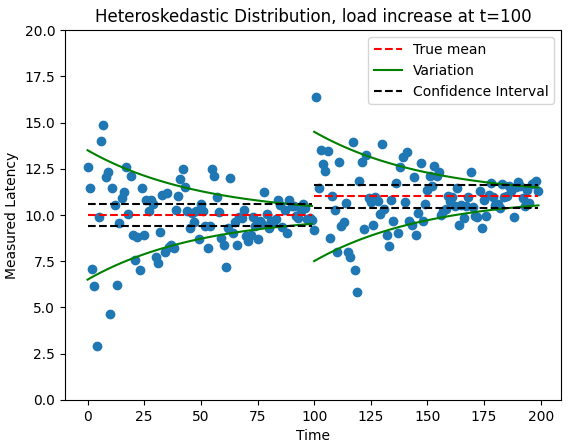
\includegraphics[width=0.7\textwidth]{distrib.png}
  \caption{Hypothetic Latency Distribution}
  \label{fig:sample}
\end{figure}

\noindent We can see on the graph that with time, variance decreases as transient latency settles down. At time $t=100$, we have reached our confidence interval, at which point we decide that it is safe to increase the workload. This change causes the variance to increase again, before settling down to a new maximum. We iterate through this process, until we have good statistical certainty that we have reached maximum throughput within a tail latency constraint. 

\noindent Compared to factor analysis, this strategy only requires us to experimentally measure latency from our system which we treat as a black box. This however raises some new theoretical questions which we explain in the next section.

\singlespacing

\noindent \textit{Related Work:} As explained in the Stage 1 report, and after further investigation, we find a large amount of literature around tail latency, its characterization and its sources. Once again, our purpose is different from those papers since we are in a testing environment in which we have control over the system load, unlike in production.


\section{Questions, Hypotheses and Test}

\textit{Hypothesis:} Although we have abandoned factor analysis, we persist with the same hypothesis, which we believe to be valid. We however use a different method to achieve this goal.

\singlespacing

\noindent \textit{Questions:} There are two main theoretical problems which we need to solve.

\singlespacing 

What interval to precisely measure the distribution ? Provided tools enable to accurately measure latency for a given number of samples, however in our case that number of samples is undefined.


What interval until we have converged to the inherent distribution ?

The tools to measure latency assume a constant distribution

\noindent 1. Since we are continuously evaluating our model, at any given time, we need to determine how large should our samples should be for accurate latency measurement.

• New questions, for instance, anomalies encountered during experiments or literature review.
\singlespacing

\noindent \textit{Testing:} There are two main theoretical problems which we need to solve.

• Methodology details, including machine configuration, software usage, and benchmarks to be conducted.

We have chosen the silo workload

\section{Progress, Result and Analysis}

Results may vary with the type of research question. Below are suggestions for a given type of research question:

• Metric Modeling: Include your model, analysis steps, experimental validation results, and error analysis.

• Solution Proposal: Test results supporting your design decisions.

• Result Reproduction: Experimental findings and comparisons with previous studies.

• Workload Characterization: Measurements of metrics.

• Methodology Examination: Comparative measurements using different methodologies.

\singlespacing
Detail the algorithm for throughput maximization

\section{Challenges}

Segmentation faults, huge codebase which is not up to date, does not compile out of the box, when it does compile, segmentation faults which need to be fixed with GDB.

Workload is not continuous - performance hysteresis - want to optimize for a single run

• Difficulties encountered, whether in experimentation, data gathering, or literature review.

• Assistance requests for your project.
\section{Plan}

• Updates on team composition (e.g., team member changes).

• Reprioritization of questions, hypotheses, and tests.

• Schedule adjustments (compared to the initial proposal).

• Updates on the final goal (compared to the initial proposal).


%\bibliographystyle{IEEEtran}
%\bibliography{ref}

\end{document}
